% content.tex - 正文内容
\section{提出问题}
\subsection{提出问题一}
\subsubsection{三级标题}
正文内容...\cite{ref1}\cite{ref2}

% 图片示例
\begin{figure}[htbp]
    \centering
    \subfigure[图题]{
        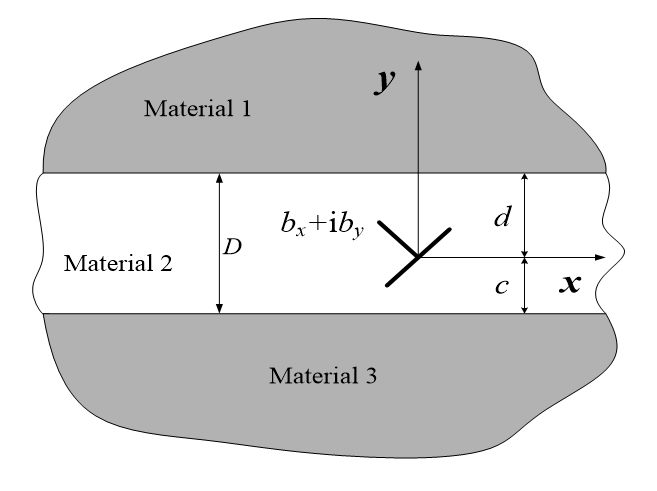
\includegraphics[width=0.45\textwidth]{figure/example.jpg}
    }
    \subfigure[图题]{
        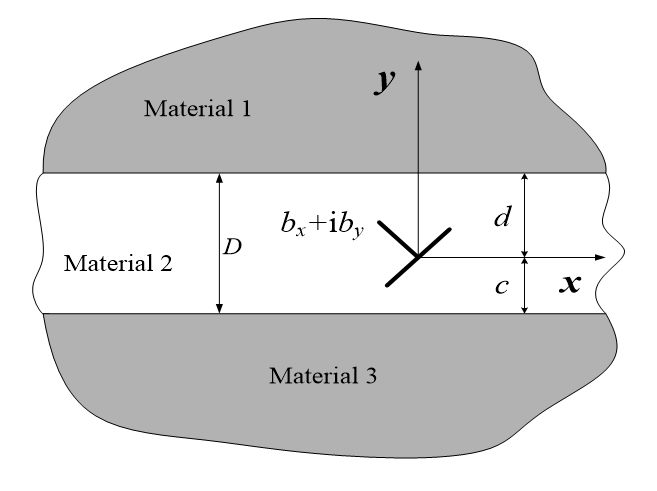
\includegraphics[width=0.45\textwidth]{figure/example.jpg}
    }
    \caption{位于三层材料体系中的位错示意图}
    \label{fig:dislocation}
\end{figure}

% 表格示例
\begin{table}[htbp]
    \centering
    \caption{表题}
    \label{tab:example}
    \begin{tabular}{ccc}
        \toprule
        速度/(m.s\textsuperscript{-1}) & 时间/s & 频率/kHz \\
        \midrule
        第一次 & ... & ... \\
        第二次 & ... & ... \\
        第三次 & ... & ... \\
        \bottomrule
    \end{tabular}
\end{table}

% 公式示例
\begin{equation}
    E = mc^2
    \label{eq:example}
\end{equation}

% ==================================